\documentclass[a4paper,11pt]{article}

\usepackage[margin=1in]{geometry}
\usepackage{amsmath,amssymb,amsfonts,bm}
\usepackage{booktabs,multirow,array,tabularx}
\usepackage{graphicx}
\usepackage{float}
\usepackage{caption}
\usepackage{subcaption}
\usepackage{pgfplots}
\pgfplotsset{compat=1.18}
\captionsetup[figure]{font=small,labelfont=bf}
\captionsetup[table]{font=small,labelfont=bf}
\usepackage{hyperref}
\usepackage{xcolor}
\usepackage{enumitem}

\hypersetup{
    colorlinks=true,
    linkcolor=blue,
    citecolor=blue,
    urlcolor=blue
}

\newcommand{\R}{\mathbb{R}}
\newcommand{\DeltaW}{\Delta W}
\newcommand{\Wzero}{W_0}
\newcommand{\rank}{\operatorname{rank}}

\title{TiRA: Tiled Rank-1 Adaptation for High-Rank Parameter-Efficient Fine-Tuning}
\author{}
\date{}

\makeatletter
\let\ps@plain\ps@empty
\makeatother

\begin{document}
\pagestyle{empty}
\maketitle

\begin{abstract}
Pre-trained large language models (LLMs) exhibit strong general language capabilities, yet they still require task-specific adaptation for complex downstream applications. Full-parameter fine-tuning is often expensive in computation and storage, whereas parameter-efficient fine-tuning (PEFT) reduces training cost by optimizing only a small number of additional parameters. As a representative PEFT method, LoRA performs adaptation through low-rank decomposition, but the effective dimensionality of its update space is constrained by the fixed rank $r$. This limitation can lead to insufficient update rank in complex adaptation scenarios. To address this issue, this paper proposes TiRA (Tiled Rank-1 Adaptation), a tiled high-rank adaptation method. TiRA partitions the weight update matrix into an $M\times M$ grid of sub-blocks and uses $K$ groups of short-vector outer products to fill shifted block diagonals in a structured manner. Under the same trainable-parameter budget as LoRA, TiRA can increase the effective rank from $r$ to $r^2$, thereby providing a higher-dimensional adaptation space for complex tasks. TiRA remains mergeable with the original weights and therefore introduces no additional inference-time overhead. We systematically evaluate TiRA on commonsense reasoning, open-domain dialogue generation, and mathematical reasoning. Experimental results show that, under matched trainable-parameter budgets, TiRA outperforms representative PEFT methods including LoRA, DoRA, MoRA, and HiRA on Llama-2-7B and Llama-3-8B. In particular, on GSM8K with Llama-3-8B, TiRA achieves $73.01\%$ accuracy, improving over LoRA by $7.12$ percentage points and over HiRA by $2.20$ percentage points. Further sensitivity analyses show that the tiling granularity $M$ has a substantial effect on TiRA, and larger models generally benefit more from high-rank adaptation. These findings validate structured tiled high-rank updates as an effective route toward efficient adaptation of LLMs for complex downstream tasks. The code and experimental data are available at \url{https://github.com/loop-xxx/TiRA}.
\end{abstract}

\section{Introduction}

Pre-trained large language models have strong general-purpose language capabilities, but their original parameters are often not directly suited to specific downstream tasks. Full-parameter fine-tuning can improve task performance, yet it incurs substantial memory, computation, and storage costs. Parameter-efficient fine-tuning mitigates this problem by freezing the backbone model and optimizing only a small set of newly introduced parameters. Existing PEFT methods can be broadly divided into prompt-based methods and reparameterization-based methods. Prompt-based methods steer model behavior by introducing trainable soft prompts or virtual tokens, whereas reparameterization-based methods, represented by LoRA \cite{hu2022lora}, reparameterize task-specific weight increments in internal linear layers. Compared with prompt-based methods, LoRA does not consume additional context length, and its low-rank weight update can be merged into the base weights before inference. It has therefore become an important paradigm in PEFT research.

However, the central assumption behind LoRA is that the weight update has a low-rank structure. This design is effective for relatively simple task adaptation, but in complex downstream tasks, the low-dimensional update subspace spanned by a fixed rank $r$ may be insufficient to represent the required high-dimensional weight changes. Directly increasing the LoRA rank can increase the dimensionality of the update space, but it also increases the number of trainable parameters, memory footprint, and optimization cost, thereby weakening the efficiency advantage of PEFT. This paper therefore asks the following question: can we construct a weight-update form with a higher effective rank while preserving the same trainable-parameter scale as LoRA and retaining mergeability with the original weights?

To answer this question, we propose TiRA, a tiled high-rank adaptation method. TiRA inherits the side-branch adaptation paradigm of LoRA, but it no longer applies a global low-rank decomposition to the entire weight update matrix. Specifically, TiRA partitions the update matrix $\DeltaW$ into an $M\times M$ block grid and organizes the trainable parameters into $K$ low-rank groups. Each group uses $M$ pairs of short-vector outer products to generate $M$ rank-1 sub-blocks along a shifted block diagonal, as illustrated in Fig.~\ref{fig:lora_tira}. This design gives each group a submatrix whose rank is upper-bounded by $M$, and the update matrix obtained by summing $K$ groups can reach a rank upper bound of $KM$. When $K=M=r$, TiRA uses $r(d_{\mathrm{out}}+d_{\mathrm{in}})$ parameters, exactly matching LoRA, while increasing the effective rank from $r$ to $r^2$. It thus achieves a quadratic rank expansion under the same parameter budget.

\begin{figure}[H]
    \centering
    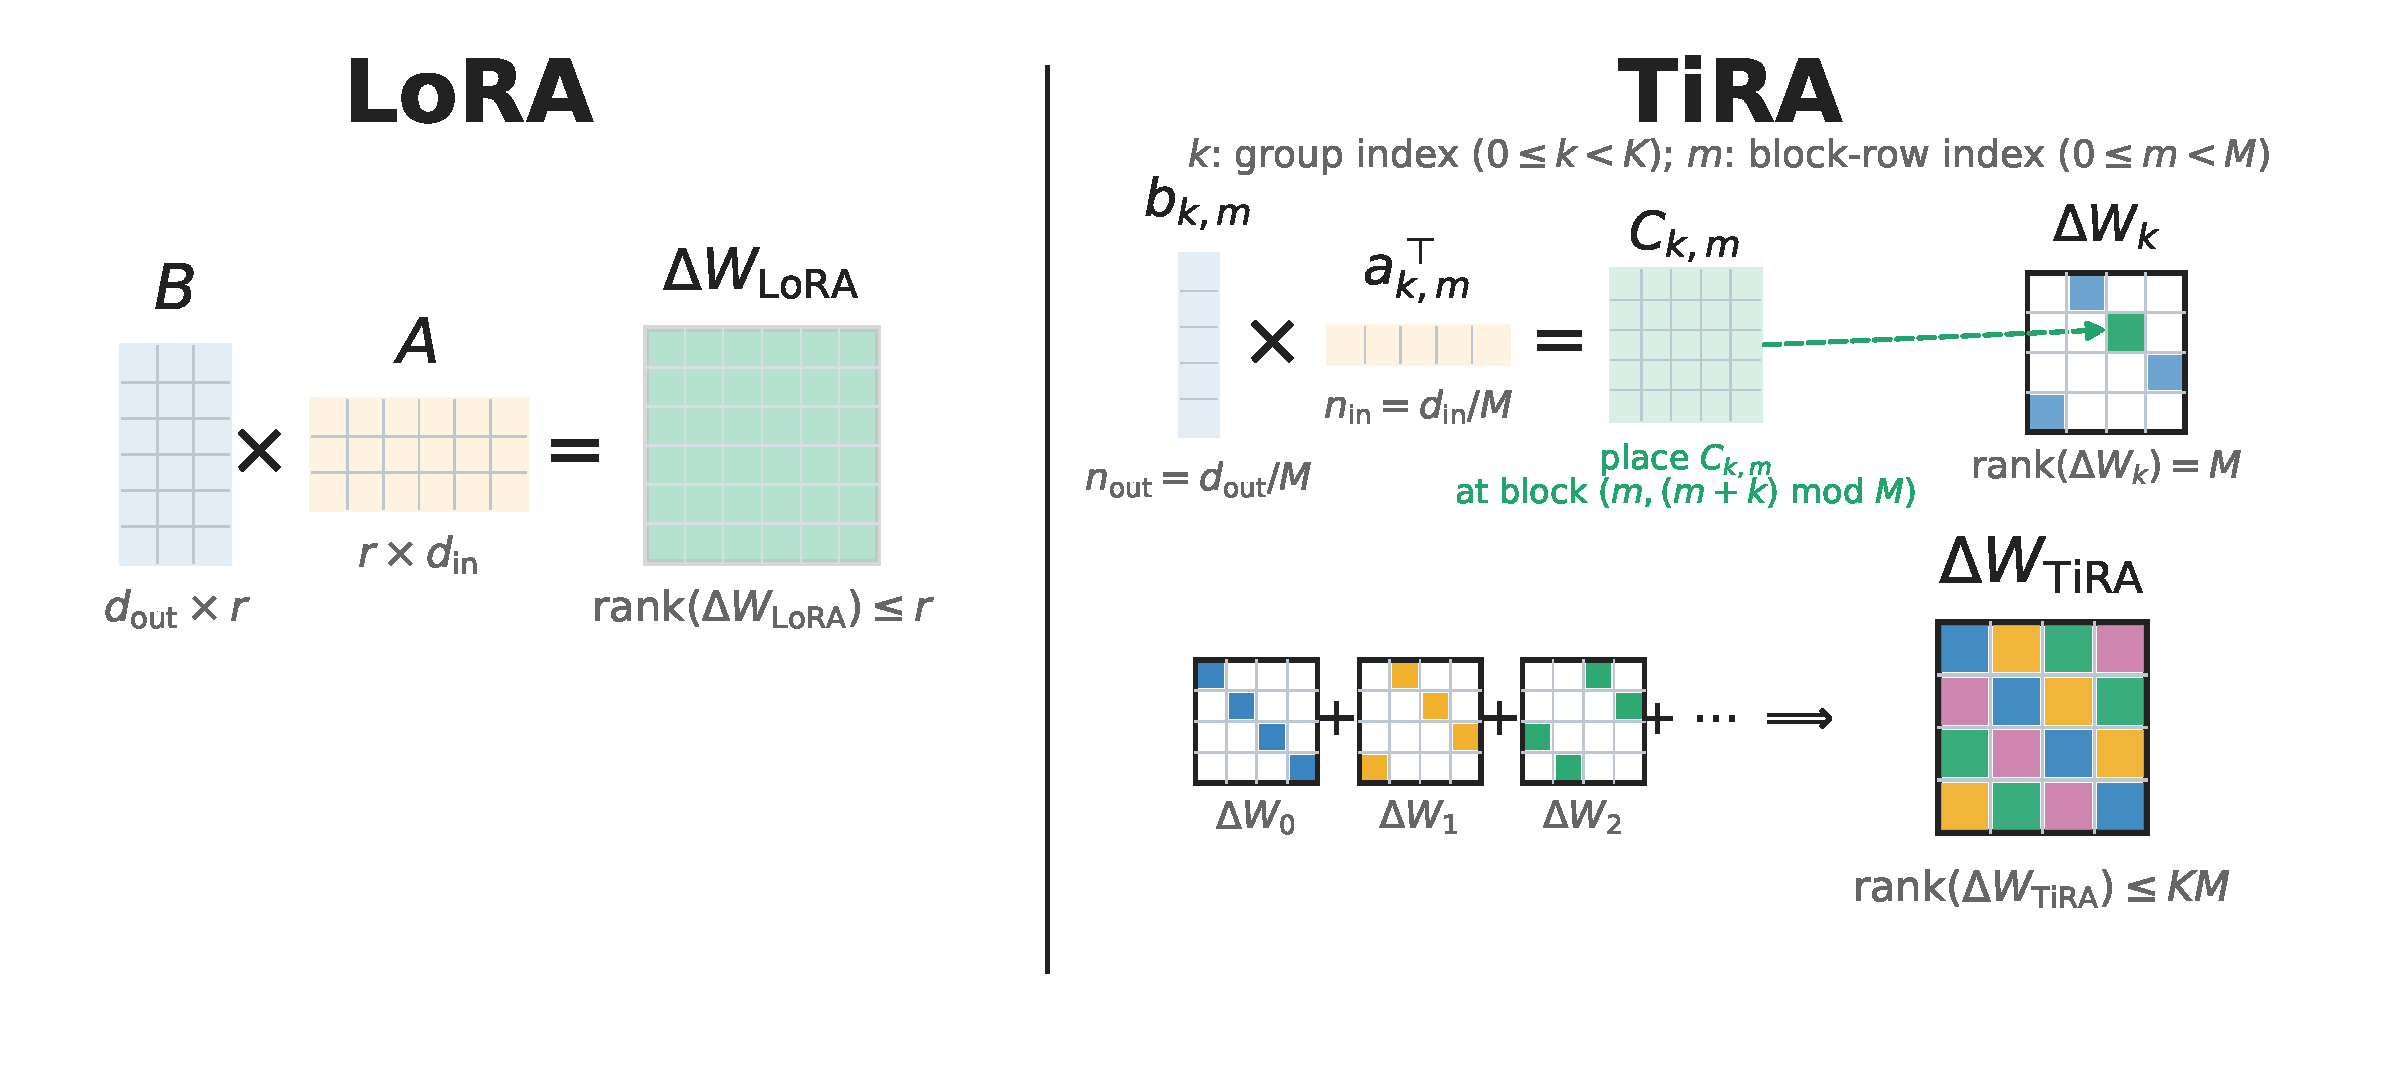
\includegraphics[width=0.96\linewidth]{figures/lora_tira_architecture.pdf}
    \caption{Architectural comparison between LoRA and TiRA. LoRA constructs the weight update $\Delta W$ using the low-rank factorization $BA$, whose rank is upper-bounded by $r$. TiRA partitions $\Delta W\in\R^{d\times d}$ into an $M\times M$ block grid, uses $K$ groups of trainable short vectors to generate rank-1 sub-blocks through outer products, and fills the update matrix along $K$ shifted block diagonals. Here, $W_0$ denotes the frozen original weight, and $K$ and $M$ are the key TiRA hyperparameters controlling parameter grouping and tiling granularity.}
    \label{fig:lora_tira}
\end{figure}

Multi-step mathematical reasoning typically requires the model to perform long chains of intermediate derivations \cite{wei2022cot,kojima2022zero}, and the task complexity increases substantially with reasoning depth. To further examine whether complex tasks require higher adaptation rank, we construct Easy and Challenge subsets from the GSM8K \cite{cobbe2021gsm8k} training set according to answer length. Longer answers usually correspond to longer reasoning chains and higher reasoning difficulty. We split each subset into training and validation sets with a $9:1$ ratio and conduct a rank comparison experiment. The hyperparameters are listed in Appendix~\ref{app:lora_hyperparams}. As shown in Fig.~\ref{fig:rank_motivation}, accuracy on the Easy subset rises rapidly at low ranks, from $56.80\%$ at $r=8$ to $67.47\%$ at $r=32$, and then slightly decreases as the rank continues to increase, reaching $65.07\%$ at $r=128$. This behavior indicates early saturation and high-rank redundancy. In contrast, the Challenge subset improves only marginally in the low-rank regime, with $42.90\%$ accuracy at $r=8$, $r=16$, and $r=32$, but continues to improve at higher ranks and reaches $47.45\%$ at $r=128$. These results suggest that more complex tasks place stronger demands on a higher-dimensional update space and therefore require higher adaptation ranks.

\begin{figure}[H]
    \centering
    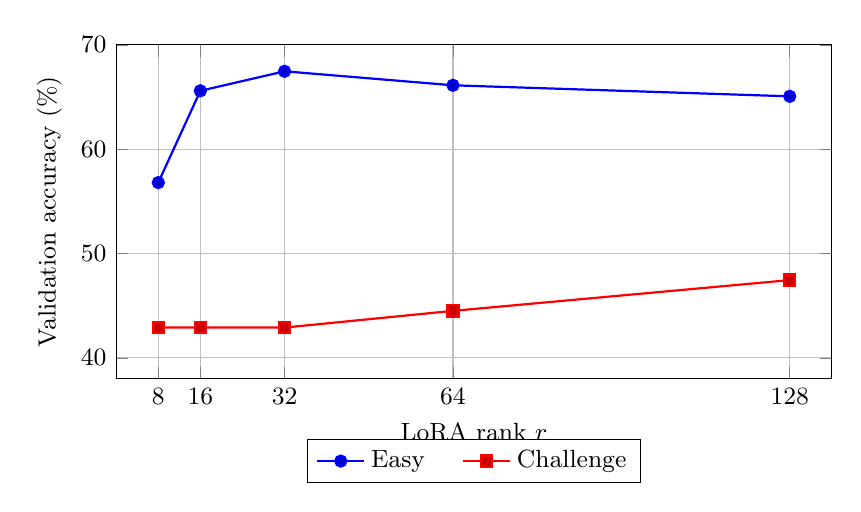
\begin{tikzpicture}
    \begin{axis}[
        width=0.88\linewidth,
        height=0.48\linewidth,
        xlabel={LoRA rank $r$},
        ylabel={Validation accuracy (\%)},
        xmin=0, xmax=136,
        ymin=38, ymax=70,
        xtick={8,16,32,64,128},
        grid=both,
        tick label style={font=\small},
        label style={font=\small},
        legend style={
            at={(0.5,-0.18)},
            anchor=north,
            legend columns=2,
            font=\small,
            /tikz/every even column/.append style={column sep=0.4cm}
        },
    ]
    \addplot+[blue, thick, mark=*] coordinates {
        (8,56.80) (16,65.60) (32,67.47) (64,66.13) (128,65.07)
    };
    \addplot+[red, thick, mark=square*] coordinates {
        (8,42.90) (16,42.90) (32,42.90) (64,44.50) (128,47.45)
    };
    \legend{Easy, Challenge}
    \end{axis}
    \end{tikzpicture}
    \caption{Validation accuracy of Qwen-2-1.5B fine-tuned with different LoRA ranks $r$ on the GSM8K Easy and Challenge subsets. The horizontal axis denotes the LoRA rank, and the vertical axis denotes validation accuracy (\%).}
    \label{fig:rank_motivation}
\end{figure}

The main contributions of this paper are as follows:
\begin{enumerate}[leftmargin=2em]
    \item We propose TiRA, a high-rank parameter-efficient adaptation method for large language models. Under a parameter budget strictly matched to LoRA, TiRA increases the effective rank of the weight update from $r$ to $r^2$, thereby providing a higher-dimensional update space and improving performance on complex downstream tasks.
    \item We introduce a decoupled hyperparameter configuration for TiRA and systematically analyze the relationship between the optimal tiling granularity and model scale. By decoupling the group number $K$ from the tiling granularity $M$, TiRA allows the parameter budget and the high-rank structure to be adjusted independently. Experiments show that the optimal $M$ generally shifts to larger values as the model scale increases, while an excessively large tiling granularity may lead to a rank-overload effect.
    \item We validate TiRA across multiple downstream task categories. The results show that TiRA preserves parameter efficiency and zero additional inference overhead while outperforming representative PEFT baselines on commonsense reasoning, open-domain dialogue generation, and mathematical reasoning.
\end{enumerate}

\section{Related Work}

\subsection{LoRA and Its Extensions}

Low-Rank Adaptation (LoRA) is a classical reparameterization-based PEFT paradigm \cite{hu2022lora}. It freezes the parameters of the pre-trained backbone and injects a pair of trainable low-rank matrices into linear layers as adapters, using the matrix product $BA$ to approximate the weight update $\DeltaW$. A key advantage of LoRA is its mathematical compatibility with the base model weights. After fine-tuning, the side-branch parameters can be explicitly folded into a weight update and merged with the original weight matrix as $W=W_0+\DeltaW$. Thus, deployment does not require an additional side branch, and the forward computation has the same form as the original linear layer, introducing no extra inference latency or memory cost.

DoRA \cite{liu2024dora} improves low-rank adaptation from the perspective of weight decomposition. It explicitly decomposes pre-trained weights into magnitude and direction components and models their changes separately during fine-tuning. The magnitude component is directly updated as trainable parameters, whereas the direction component follows the low-rank update mechanism of LoRA. By separately adjusting weight magnitude and direction, DoRA can more closely approximate the weight-change pattern of full fine-tuning with a small parameter overhead. Its directional update can still be merged with the base weights before inference, preserving LoRA's deployment advantage of no additional inference latency.

Another line of work directly addresses the low-dimensional update-space limitation caused by LoRA's low-rank update and introduces high-rank weight updates under PEFT constraints. MoRA \cite{jiang2024mora} argues that low-rank updates may limit the model's ability to learn and memorize new knowledge. It therefore uses square adapters together with non-parametric compression and expansion operators to increase the update rank while keeping the trainable-parameter count comparable. However, its static mapping functions make direct merging between adapter weights and original weights more complicated. HiRA \cite{huang2025hira} constructs high-rank adaptation through the Hadamard product. It first obtains a low-rank matrix $BA$ from trainable matrices $B$ and $A$, and then multiplies it element-wise with the frozen pre-trained weight matrix $W_0$, namely $\DeltaW = W_0 \odot (BA)$. Since the Hadamard product satisfies $\rank(P\odot Q)\leq \rank(P)\rank(Q)$, the final update $\DeltaW$ may have a higher rank upper bound when $W_0$ itself has high rank, even if $BA$ remains low-rank. HiRA therefore increases update-space dimensionality while maintaining a trainable-parameter count close to LoRA, and it can merge the adapter weights into the pre-trained weights before inference.

\subsection{Other PEFT Methods}

Another important class of PEFT methods is prompt-based adaptation. These methods embed trainable virtual tokens into the input layer or hidden layers of an LLM and optimize only the prompt parameters while keeping the backbone parameters frozen. Representative methods include Prefix Tuning \cite{li2021prefix}, Prompt Tuning \cite{lester2021power}, and P-Tuning v2 \cite{xiao2022ptuning}. Prompt Tuning prepends soft prompts to the input sequence for task adaptation. Prefix Tuning injects trainable prefixes into the attention computation. P-Tuning v2 further extends continuous prompts to deeper representation spaces, improving the ability to control complex task patterns. The performance of this family of methods is often sensitive to prompt length, initialization, and task format. Unlike LoRA and its variants, which directly modify internal linear projections, prompt-based methods mainly induce task-specific outputs by altering the input or intermediate representation space.

\section{Method}

\subsection{Side-Branch Adaptation Framework}

LoRA implements parameter-efficient fine-tuning for linear projection modules in neural networks. Since Transformer \cite{vaswani2017attention} has become the dominant architecture for modern LLMs, its Query, Key, Value, and Output projection matrices, as well as the projection layers in its feed-forward network, are natural targets for LoRA because they are linear projections. LoRA freezes all pre-trained weights and introduces low-rank side-branch matrices only alongside linear projection layers as trainable adapters. For an original weight matrix $W\in\R^{d_{\mathrm{out}}\times d_{\mathrm{in}}}$, LoRA trains two low-rank matrices $B\in\R^{d_{\mathrm{out}}\times r}$ and $A\in\R^{r\times d_{\mathrm{in}}}$ and adjusts the original linear projection as
\begin{equation}
    W_{\mathrm{merged}} = W + BA .
\end{equation}
This design is convenient for deployment. After fine-tuning, the side-branch parameters can be merged into the original weights by matrix addition, avoiding extra inference latency and memory overhead.

\subsection{Core Idea and Formal Construction of TiRA}

TiRA follows the side-branch adaptation framework of LoRA but breaks the global low-rank constraint through a tiled construction. Instead of decomposing the entire weight update matrix with rank $r$, TiRA partitions the update matrix $\DeltaW\in\R^{d_{\mathrm{out}}\times d_{\mathrm{in}}}$ into $M\times M$ unit blocks. Each unit block has size $n_{\mathrm{out}}\times n_{\mathrm{in}}$, where $n_{\mathrm{out}}=d_{\mathrm{out}}/M$ and $n_{\mathrm{in}}=d_{\mathrm{in}}/M$. Each used unit block is assigned an independent rank-1 adapter.

Specifically, the rank-1 adapters are divided into $K$ groups. The $k$-th group ($0\leq k<K$) contains $M$ pairs of trainable short vectors:
\begin{equation}
    \{\bm{b}_{k,m},\bm{a}_{k,m}\}_{m=0}^{M-1},\quad
    \bm{b}_{k,m}\in\R^{n_{\mathrm{out}}},\quad
    \bm{a}_{k,m}\in\R^{n_{\mathrm{in}}}.
\end{equation}
Each vector pair generates one rank-1 sub-block through an outer product:
\begin{equation}
    C_{k,m}=\bm{b}_{k,m}\bm{a}_{k,m}^{\top}\in\R^{n_{\mathrm{out}}\times n_{\mathrm{in}}}.
\end{equation}
TiRA constructs the complete update matrix with a shifted block-diagonal grouping strategy. The $k$-th adapter group occupies one shifted block diagonal: the $m$-th rank-1 sub-block is placed in block row $m$ and block column $(m+k)\bmod M$, while all other block positions are set to zero. The sparse update matrix of the $k$-th group is therefore
\begin{equation}
    [\Delta W_k]_{i,j}=
    \begin{cases}
        C_{k,m}, & i=m,\; j=(m+k)\bmod M,\\
        0, & \text{otherwise}.
    \end{cases}
\end{equation}
Summing over all groups gives the total weight update:
\begin{equation}
    \DeltaW = \sum_{k=0}^{K-1}\Delta W_k .
\end{equation}
When $K=M$, the $M$ shifted block diagonals exactly cover all $M\times M$ block positions, and each block position is filled by a rank-1 sub-block generated from one short-vector outer product. Appendix~\ref{app:k3m3} gives a concrete example for $K=M=3$ to illustrate the shifted block-diagonal grouping strategy.

\subsection{Parameter Count and Rank Analysis}

Each group contains $M$ rank-1 sub-blocks, corresponding to $M$ pairs of trainable short vectors. Therefore, the total number of TiRA parameters is
\begin{equation}
    \mathrm{Params}=K\times M\times(n_{\mathrm{out}}+n_{\mathrm{in}})=K(d_{\mathrm{out}}+d_{\mathrm{in}}).
\end{equation}
When $K=M=r$, TiRA and LoRA have exactly the same parameter count, namely $r(d_{\mathrm{out}}+d_{\mathrm{in}})$. Their key difference lies in rank expansion: each group independently contributes a rank upper bound of $M$, and the sum of $K$ groups can reach a rank upper bound of $KM$. Thus, when $K=M=r$, TiRA increases the effective rank upper bound from LoRA's $r$ to $r^2$, thereby enhancing the model's adaptation ability in complex tasks.

The initialization follows the standard LoRA practice. The vectors $\bm{a}_{k,m}$ are initialized with Kaiming uniform initialization \cite{he2015rectifier} to maintain stable gradient flow at the beginning of training, while $\bm{b}_{k,m}$ are zero-initialized so that $\DeltaW=0$ at initialization. This preserves the initial behavior of the pre-trained model.

\subsection{Theoretical Feasibility and Optimization Equivalence}

The adaptation ability of LoRA generally improves as the rank increases, but its parameter count also grows linearly. Mathematically, a LoRA adapter with rank $K\times r$ can be written as the sum of $K$ LoRA adapters of rank $r$. Based on this observation, if a structured sparse mask is introduced for each rank-$r$ LoRA adapter so that different modules update non-overlapping and complementary subspaces, the equivalent rank may be expanded by a factor of $K$ while keeping the parameter budget of the original rank-$r$ LoRA module.

For the case $M=K=r$, the weight-update matrix produced by the $k$-th adapter module can be written as $\Delta W_k=B_kA_k^{\top}$, where $B_k\in\R^{d_{\mathrm{out}}\times M}$ and $A_k^{\top}\in\R^{M\times d_{\mathrm{in}}}$ are both structured sparse matrices. Their sparse nonzero patterns are determined by the cyclic shift indexed by $k$, so the nonzero update positions of different adapter modules are staggered and complementary. Each individual module therefore remains sparse, while their sum covers a more complete set of update positions, enlarging the overall update space under the same sparse parameter budget. We refer to this structure as multi-sparse LoRA expert adaptation and provide a concrete example for $r=3$ in Appendix~\ref{app:sparse_expert}.

TiRA and this multi-sparse LoRA expert adaptation are linear reparameterizations of the same parameter space. From an optimization perspective, they have the same parameter-space dimension and parameter count, both equal to $M(d_{\mathrm{out}}+d_{\mathrm{in}})$, and they reach exactly the same set of update matrices:
\begin{equation}
    \{\Delta W_{\mathrm{block}}(\theta)\mid \theta\in\R^{M(d_{\mathrm{out}}+d_{\mathrm{in}})}\}
    =
    \{\Delta W_{\mathrm{expert}}(\theta)\mid \theta\in\R^{M(d_{\mathrm{out}}+d_{\mathrm{in}})}\}.
\end{equation}
The two indexing rules from parameters to matrix entries can be converted into each other through a linear bijection $T$, i.e., a permutation matrix satisfying $T^{\top}T=I$. For any parameter assignment $\theta$, the update generated by TiRA is equivalent to the expert form under the transformed parameters $T\theta$:
\begin{equation}
    \Delta W_{\mathrm{block}}(\theta)=\Delta W_{\mathrm{expert}}(T\theta).
\end{equation}
TiRA groups parameters from the same group contiguously along the $(m+k)\bmod M$ block diagonal, forming a locally dense block-sparse structure. The expert form instead interleaves parameters across the global matrix according to modulo-$M$ congruence classes, forming a globally sparse structure. By the chain rule, the gradients under the two parameterizations satisfy
\begin{equation}
    \nabla_{\theta}\mathcal{L}_{\mathrm{block}}
    =T^{\top}\nabla_{\phi}\mathcal{L}_{\mathrm{expert}}\big|_{\phi=T\theta}.
\end{equation}
Because $T$ only permutes parameter coordinates, the two forms do not change the reachable set of weight updates or the fundamental relation between gradient directions. Under the same initialization and training settings, they can therefore be regarded as two equivalent parameterizations of the same structured update space and are expected to exhibit similar optimization behavior.

In summary, TiRA inherits the theoretical feasibility and higher-dimensional adaptation space of multi-sparse LoRA expert adaptation. At the same time, its contiguous tiled structure better matches GPU memory locality and can implement the forward pass through efficient block matrix multiplication, avoiding the extra overhead associated with sparse indexing.

\subsection{Decoupled Hyperparameter Configuration}

TiRA decouples the hyperparameters $K$ and $M$: $M$ mainly determines the tiling granularity, while $K$ mainly determines the actual parameter count and the effective rank within each block. This decoupling allows TiRA to increase update-space dimensionality by adjusting $K$ without changing the tiling structure, making it flexible under different compute budgets. To use all $M$ diagonal bands evenly, $K$ should satisfy $K\geq M$ and be an integer multiple of $M$:
\begin{equation}
    K=L\cdot M,
\end{equation}
where $L\in\mathbb{Z}^{+}$ denotes the number of stacked components at each block position. When $L=1$ (i.e., $K=M$), each diagonal band corresponds to one adapter group. When $L\geq2$, TiRA enters a multi-layer accumulation mode, where the parameter count, within-block rank, and total rank upper bound increase with $L$. If $M$ is fixed and the compute budget allows a higher-dimensional update space, $K$ can be set to a multiple of $M$, such as $K=2M,3M,\ldots$. Each group $k$ still follows the cyclic-shift diagonal placement rule, while the rank-1 sub-blocks from $L$ groups are summed at each position on the same diagonal band. Appendix~\ref{app:m3k6} gives a construction example for $M=3,K=6$ ($L=2$).

Under this construction, each unit block contains the sum of $L$ independent short-vector outer products, and its effective rank upper bound increases from 1 to $L$. Therefore, the total rank upper bound is
\begin{equation}
    \rank(\DeltaW)\leq \min\{M^2L,\;d_{\mathrm{out}},\;d_{\mathrm{in}}\}.
\end{equation}
Thus, when $M$ is fixed, increasing $L$ improves the within-block effective rank through multi-layer accumulation and makes the total rank upper bound grow approximately linearly with $L$.

In the special case $M=1$, TiRA no longer partitions the weight update matrix. Then $L=K$, and $\DeltaW$ is the sum of $K$ rank-1 outer-product matrices, which is equivalent to the low-rank decomposition $\DeltaW=BA$, where $B\in\R^{d_{\mathrm{out}}\times K}$ is formed by concatenating $\{\bm{b}_k\}$ as columns and $A\in\R^{K\times d_{\mathrm{in}}}$ is formed by stacking $\{\bm{a}_k^{\top}\}$ as rows.

\section{Experiments}

To comprehensively evaluate the adaptation capability of TiRA on heterogeneous tasks, we conduct experiments on commonsense reasoning, open-domain dialogue generation, and mathematical reasoning.

\subsection{Datasets}

The commonsense reasoning experiments follow the setting of LLM-Adapters \cite{hu2023llmadapters}. Multiple commonsense reasoning datasets are combined into a unified training set, from which 120 samples are randomly selected as the validation set. We evaluate model performance on eight commonsense reasoning subtasks, with 170,420 question-answer samples used for fine-tuning. The subtasks include BoolQ \cite{bisk2019boolq}, PIQA \cite{bisk2020piqa}, SIQA \cite{sap2019socialiqa}, HellaSwag \cite{zellers2019hellaswag}, WinoGrande \cite{sakaguchi2021winogrande}, ARC-e, ARC-c \cite{clark2018arc}, and OBQA \cite{mihaylov2018openbookqa}. BoolQ evaluates Boolean question answering; PIQA focuses on physical commonsense reasoning; SIQA concerns social commonsense reasoning; HellaSwag targets commonsense natural language inference; WinoGrande evaluates pronoun resolution and commonsense judgment in a cloze-style format; ARC-e and ARC-c correspond to easy and challenging partitions of science multiple-choice questions; and OBQA emphasizes open-book multi-step commonsense reasoning.

The open-domain dialogue generation experiments are conducted on ConvAI2 \cite{dinan2019convai2}. Each multi-turn dialogue in this dataset is accompanied by a persona composed of 4--5 descriptive sentences and dialogue history. Following prior experimental settings, we provide only the current speaker's own persona to the model and do not include the interlocutor's persona. This evaluates the model's ability to generate coherent and natural responses conditioned on its own persona and the dialogue context.

For mathematical reasoning, we use MetaMath \cite{yu2024metamath} as the training corpus and evaluate on the original GSM8K \cite{cobbe2021gsm8k} test set. MetaMath is constructed by reasoning-oriented augmentation and rewriting of mathematical datasets such as GSM8K and MATH, providing richer multi-step reasoning training examples. GSM8K consists of grade-school math word problems and requires step-by-step derivation of final numerical answers, making it a standard benchmark for mathematical reasoning and generalization in LLMs.

\subsection{Experimental Setup}

\paragraph{Evaluation metrics.}
Commonsense reasoning is evaluated with accuracy. The model generates free-form text responses from the input query, and predicted answers are extracted from the generated text through keyword matching. For example, BoolQ recognizes ``true'' or ``false'', whereas multiple-choice tasks match predefined candidate-answer keywords for each dataset. For each sample, the first matched valid keyword is treated as the prediction; if no target keyword is detected, the prediction is counted as incorrect. This evaluation process follows DoRA and HiRA. Open-domain dialogue generation is evaluated with automatic generation-quality metrics, including BLEU \cite{papineni2002bleu}, METEOR \cite{banerjee2005meteor}, ROUGE-L \cite{lin2004rouge}, and BERTScore \cite{zhang2019bertscore}. Mathematical reasoning follows the standard practice of accuracy-based evaluation. The generated final answer is matched against the gold answer. In implementation, we extract both the last numerical value in the generated text and the numerical value after an explicit answer cue, and compare each with the gold answer. A sample is counted as correct if either extraction matches the gold answer.

\paragraph{Baselines.}
We compare TiRA with representative PEFT methods covering both prompt tuning and low-rank adaptation. The prompt-tuning baselines include Prompt Tuning and P-Tuning; the low-rank adaptation baselines include LoRA, DoRA, MoRA, and HiRA. All main experiments are conducted on two open-source LLMs, Llama-2-7B \cite{touvron2023llama2} and Llama-3-8B \cite{grattafiori2024llama3}. Except for the TiRA results reproduced in this work and the LoRA controls in the tiling-granularity analysis, the main baseline results are taken from the public HiRA report to ensure comparability with prior work.

\paragraph{Implementation details.}
To maintain comparability with prior work, we adopt the same training configuration as HiRA and only adjust the learning rate for different tasks. We use the AdamW optimizer with 100 warmup steps. Commonsense reasoning is fine-tuned for 2 epochs with a learning rate of $2\times10^{-4}$, and validation is performed every 80 steps to select the best checkpoint. Open-domain dialogue generation is trained for 1 epoch with a learning rate of $2\times10^{-5}$. Mathematical reasoning is trained for 2 epochs with a learning rate of $4\times10^{-5}$. TiRA adapters are applied to the Query, Key, and Value projection matrices in the attention module, as well as the up-projection and down-projection layers in the feed-forward network. Detailed hyperparameters are provided in Appendix~\ref{app:tira_hyperparams}. To ensure a fair comparison with LoRA, DoRA, MoRA, and HiRA, we strictly control the trainable-parameter counts to the same scale.

\subsection{Commonsense Reasoning Results}

\begin{table}[H]
\centering
\small
\caption{Accuracy comparison of PEFT methods on commonsense reasoning datasets. Baseline results except TiRA are taken from HiRA. The best results are shown in bold.}
\label{tab:commonsense}
\resizebox{\textwidth}{!}{%
\begin{tabular}{llcccccccccc}
\toprule
Model & Method & Params (\%) & BoolQ & PIQA & SIQA & ARC-c & ARC-e & OBQA & HellaS & WinoG & Avg. \\
\midrule
\multirow{7}{*}{Llama-2-7B}
& Prompt Tuning & 0.0012 & 55.93 & 12.35 & 30.50 & 6.06 & 8.63 & 9.40 & 6.91 & 40.57 & 21.29 \\
& P-Tuning & 0.7428 & 58.75 & 36.02 & 0.20 & 0.17 & 1.98 & 0.80 & 0.01 & 0.00 & 12.24 \\
& LoRA ($r=32$) & 0.8256 & 69.80 & 79.90 & 79.50 & 64.70 & 79.80 & 81.00 & 82.60 & 82.60 & 77.61 \\
& DoRA ($r=32$) & 0.8256 & 71.80 & 83.70 & 76.00 & 68.20 & 83.70 & 82.40 & 89.10 & 82.60 & 79.69 \\
& MoRA ($r=32$) & 0.8241 & 72.17 & 80.79 & 79.53 & 71.42 & 85.31 & 81.20 & 29.09 & 80.19 & 72.46 \\
& HiRA ($r=32$) & 0.8256 & 71.22 & 83.35 & 79.53 & 73.81 & 86.74 & 84.60 & 88.12 & 83.98 & 81.42 \\
& TiRA ($K=M=32$) & 0.8256 & 70.86 & 83.62 & 80.71 & 72.95 & \textbf{87.67} & 84.40 & 88.98 & \textbf{84.61} & \textbf{81.72} \\
\midrule
\multirow{7}{*}{Llama-3-8B}
& Prompt Tuning & 0.0010 & 56.85 & 45.05 & 36.13 & 31.57 & 32.74 & 29.20 & 14.01 & 50.12 & 36.96 \\
& P-Tuning & 0.6240 & 59.97 & 11.64 & 8.19 & 7.42 & 8.63 & 9.60 & 1.77 & 37.65 & 18.11 \\
& LoRA ($r=32$) & 0.7002 & 70.80 & 85.20 & 79.90 & 71.20 & 84.20 & 79.00 & 91.70 & 84.30 & 80.79 \\
& DoRA ($r=32$) & 0.7002 & 74.60 & 89.30 & 79.90 & 80.40 & 90.50 & 85.80 & 95.50 & 85.60 & 85.20 \\
& MoRA ($r=32$) & 0.6997 & 74.28 & 87.43 & 80.71 & 79.61 & 91.16 & 85.60 & 43.53 & 86.74 & 78.63 \\
& HiRA ($r=32$) & 0.7002 & 75.40 & \textbf{89.70} & 81.15 & 82.90 & 93.27 & 88.32 & 95.36 & 87.70 & 86.72 \\
& TiRA ($K=M=32$) & 0.7002 & \textbf{75.66} & 89.66 & \textbf{83.16} & \textbf{83.70} & \textbf{93.64} & \textbf{90.00} & \textbf{95.83} & \textbf{89.11} & \textbf{87.60} \\
\bottomrule
\end{tabular}%
}
\end{table}

Table~\ref{tab:commonsense} shows that TiRA achieves the highest average accuracy on both base models and consistently outperforms the existing baselines. On Llama-2-7B, TiRA reaches an average accuracy of $81.72\%$, improving over the second-best method HiRA ($81.42\%$) by $0.30$ percentage points and over the conventional low-rank adaptation method DoRA ($79.69\%$) by $2.03$ percentage points. On Llama-3-8B, TiRA achieves $87.60\%$ average accuracy, exceeding HiRA ($86.72\%$) and DoRA ($85.20\%$) by $0.88$ and $2.40$ percentage points, respectively.

A closer look at individual subtasks shows that TiRA has stable advantages on most reasoning benchmarks. In particular, under the Llama-3-8B setting, TiRA obtains the best performance on SIQA, ARC-c, ARC-e, OBQA, HellaSwag, and WinoGrande. These results indicate that, under the same trainable-parameter constraint, TiRA alleviates the low-dimensional update-space limitation of conventional low-rank adaptation and provides a more effective fine-tuning scheme for complex commonsense reasoning.

\subsection{Open-Domain Dialogue Generation Results}

\begin{table}[H]
\centering
\small
\caption{Performance comparison of PEFT methods on the ConvAI2 open-domain dialogue generation dataset. Baseline results except TiRA are taken from HiRA. The best results are shown in bold.}
\label{tab:dialogue}
\resizebox{\linewidth}{!}{%
\begin{tabular}{llcccccccc}
\toprule
Model & Method & Params (\%) & BLEU & BERT F1 & BERT-R & BERT-P & METEOR & R-L & Avg. \\
\midrule
\multirow{7}{*}{Llama-3-8B}
& Prompt Tuning & 0.0012 & 1.45 & 82.99 & 82.99 & 83.05 & 14.72 & 13.13 & 46.39 \\
& P-Tuning & 0.7428 & 1.50 & 81.52 & 81.07 & 82.01 & 15.49 & 13.55 & 45.86 \\
& MoRA ($r=32$) & 0.8241 & 1.60 & 84.22 & 84.06 & 84.43 & 12.37 & 11.19 & 46.31 \\
& LoRA ($r=32$) & 0.8256 & 2.26 & 84.32 & 84.00 & 84.67 & 12.51 & 11.77 & 46.59 \\
& DoRA ($r=32$) & 0.8256 & 2.29 & 84.32 & 84.06 & 84.62 & 12.63 & 11.78 & 46.62 \\
& HiRA ($r=32$) & 0.8256 & 3.41 & \textbf{84.81} & 84.40 & \textbf{85.25} & 14.87 & 14.05 & 47.80 \\
& TiRA ($K=M=32$) & 0.7002 & \textbf{3.50} & 84.78 & \textbf{84.48} & 85.11 & \textbf{15.66} & \textbf{14.34} & \textbf{48.04} \\
\bottomrule
\end{tabular}%
}
\end{table}

As shown in Table~\ref{tab:dialogue}, TiRA obtains the best dialogue generation quality on Llama-3-8B, with an average score of $48.04\%$, outperforming HiRA ($47.80\%$), DoRA ($46.62\%$), LoRA ($46.59\%$), and MoRA ($46.31\%$). TiRA achieves the best scores on BLEU, METEOR, BERT-R, and ROUGE-L, while remaining competitive on BERT F1 and BERT-P. These results suggest that the tiled high-rank adaptation mechanism of TiRA can better capture complex semantic relations in open-domain dialogue contexts, improving consistency between generated and reference responses.

\subsection{Mathematical Reasoning Results}

\begin{table}[H]
\centering
\caption{Accuracy comparison of PEFT methods on mathematical reasoning. The training corpus is MetaMath, and the test benchmark is GSM8K. In the mathematical evaluation, a sample is counted as correct if either the last numerical value in the generated text or the numerical value after an explicit answer cue matches the gold answer. Baseline results except TiRA are taken from HiRA. The best result is shown in bold.}
\label{tab:math}
\begin{tabular}{llcc}
\toprule
Model & Method & Trainable (\%) & GSM8K \\
\midrule
\multirow{7}{*}{Llama-3-8B}
& Prompt Tuning & 0.0012 & 15.62 \\
& P-Tuning & 0.7428 & 2.65 \\
& LoRA ($r=32$) & 0.7002 & 65.89 \\
& DoRA ($r=32$) & 0.7002 & 66.12 \\
& MoRA ($r=32$) & 0.6997 & 67.98 \\
& HiRA ($r=32$) & 0.7002 & 70.81 \\
& TiRA ($K=M=32$) & 0.7002 & \textbf{73.01} \\
\bottomrule
\end{tabular}
\end{table}

Table~\ref{tab:math} shows that TiRA achieves $73.01\%$ accuracy on Llama-3-8B, substantially outperforming all baselines under the same trainable-parameter budget. Compared with the second-best method, HiRA ($70.81\%$), TiRA improves accuracy by $2.20$ percentage points. Compared with conventional low-rank adaptation methods LoRA ($65.89\%$) and DoRA ($66.12\%$), it improves by $7.12$ and $6.89$ percentage points, respectively. This result indicates that TiRA can substantially improve adaptation to complex multi-step mathematical reasoning without increasing the number of trainable parameters.

\subsection{Spectral Analysis of Adapter Weights}

To further analyze the high-rank properties of TiRA's weight updates from the parameter-space perspective, we perform singular value decomposition on the trained adapter weight updates $\DeltaW$ from the mathematical reasoning experiments and compare them with LoRA under the same parameter budget. Specifically, we select the best checkpoints of Llama-3-8B trained on MetaMath, construct LoRA's $\DeltaW=BA$ and TiRA's tiled $\DeltaW$, and report averaged spectral metrics over all adapter layers and target linear modules. Effective rank is computed using the singular-value threshold $\tau=0.005$. Energy rank denotes the smallest rank needed for the cumulative squared singular-value energy to reach a specified proportion, i.e., how many leading singular directions are needed to cover 95\% or 99\% of the spectral energy. A higher energy rank indicates that the weight-update energy is distributed across more adaptation directions. Stable rank is defined as $\|\DeltaW\|_F^2/\|\DeltaW\|_2^2$, which can be viewed as a continuous rank measure supported by spectral energy. If most energy is concentrated in the leading singular direction, the stable rank is small; if energy spreads across more singular directions, the stable rank increases.

\begin{table}[H]
\centering
\small
\caption{Spectral analysis of trained adapter weight updates $\DeltaW$. All metrics are averaged over the 32 layers and target modules of Llama-3-8B.}
\label{tab:delta_spectrum}
\begin{tabular}{lcccc}
\toprule
Method & Eff. rank & Stable rank & 95\% energy rank & 99\% energy rank \\
\midrule
LoRA ($r=32$) & 32.00 & 2.50 & 13.55 & 23.93 \\
TiRA ($M=16,K=32$) & 432.96 & 10.15 & 161.94 & 304.45 \\
TiRA ($M=32,K=32$) & \textbf{757.27} & \textbf{14.71} & \textbf{356.52} & \textbf{631.81} \\
\bottomrule
\end{tabular}
\end{table}

Table~\ref{tab:delta_spectrum} shows that LoRA's effective rank is strictly limited by its configured rank $r=32$, and its spectral energy is highly concentrated, with a 95\% energy rank of only 13.55. In contrast, under the same trainable-parameter count as LoRA ($r=32$), the trained TiRA updates exhibit substantially higher effective rank and more dispersed spectral energy. When $M=32,K=32$, TiRA reaches an average effective rank of 757.27 and a 95\% energy rank of 356.52, about 23.7 and 26.3 times those of LoRA, respectively. The stable rank also increases from 2.50 for LoRA to 14.71 for TiRA. These results show that TiRA's structured tiled design not only raises the theoretical rank upper bound, but also produces a higher-dimensional weight-update subspace after training.

\begin{figure}[H]
    \centering
    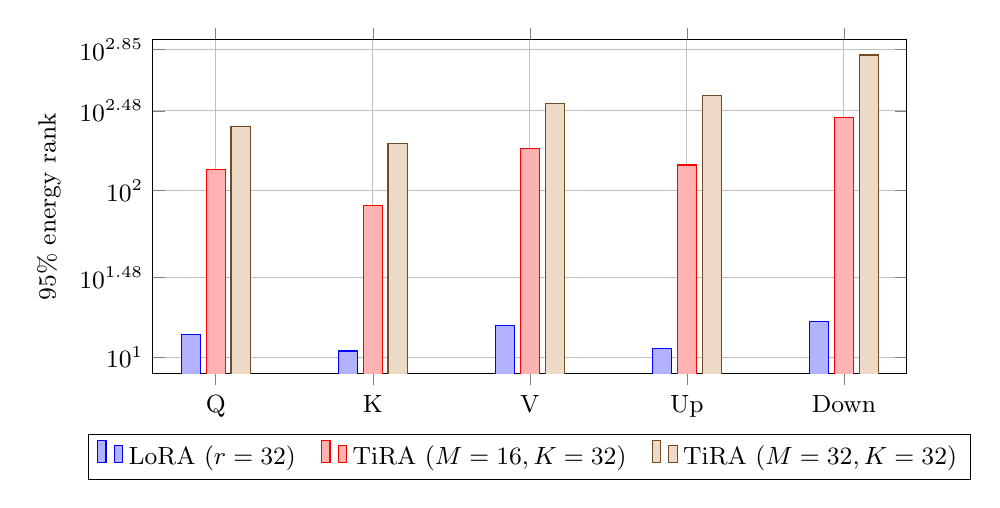
\begin{tikzpicture}
    \begin{axis}[
        ybar,
        ymode=log,
        width=0.92\linewidth,
        height=0.48\linewidth,
        bar width=7pt,
        ylabel={95\% energy rank},
        symbolic x coords={Q,K,V,Up,Down},
        xtick=data,
        ymin=8,
        ymax=800,
        ytick={10,30,100,300,700},
        grid=both,
        tick label style={font=\small},
        label style={font=\small},
        legend style={
            at={(0.5,-0.18)},
            anchor=north,
            legend columns=3,
            font=\small,
            /tikz/every even column/.append style={column sep=0.25cm}
        },
    ]
    \addplot coordinates {(Q,13.63) (K,10.91) (V,15.47) (Up,11.28) (Down,16.47)};
    \addlegendentry{LoRA ($r=32$)}
    \addplot coordinates {(Q,133.41) (K,81.53) (V,177.88) (Up,142.06) (Down,274.81)};
    \addlegendentry{TiRA ($M=16,K=32$)}
    \addplot coordinates {(Q,242.16) (K,191.69) (V,330.38) (Up,370.41) (Down,647.97)};
    \addlegendentry{TiRA ($M=32,K=32$)}
    \end{axis}
    \end{tikzpicture}
    \caption{Comparison of the 95\% energy rank of trained $\DeltaW$ across target modules. The vertical axis uses a logarithmic scale to show the order-of-magnitude differences between methods.}
    \label{fig:delta_spectrum_rank95}
\end{figure}

Figure~\ref{fig:delta_spectrum_rank95} further shows module-level spectral differences. TiRA obtains much higher 95\% energy ranks than LoRA on the Query, Key, and Value projections, as well as the up-projection and down-projection modules in the feed-forward network. This indicates that high-rank updates are not concentrated in a single layer or module, but appear consistently across the model's main linear projection modules. The gains are particularly large in the down-projection and up-projection modules, suggesting that TiRA introduces richer task-relevant perturbation directions in the feed-forward network. This qualitative analysis is consistent with the observed improvement in mathematical reasoning performance, supporting the view that TiRA's gains primarily come from the expanded update space enabled by structured high-rank updates.

\subsection{\texorpdfstring{Effect of Tiling Granularity $M$ on Adaptation Performance}{Effect of Tiling Granularity M on Adaptation Performance}}

When $M=1$, TiRA no longer partitions the matrix and degenerates to a rank-$K$ low-rank decomposition $BA$, equivalent in form to LoRA. To analyze the effect of tiling granularity $M$ on adaptation performance, we fix $K=32$ so that the number of trainable parameters in TiRA is strictly matched to LoRA ($r=32$), and vary only $M$. To further examine how the choice of tiling granularity changes with model scale, we use three open-source LLMs with increasing scale, Qwen-2-0.5B, Qwen-2-1.5B, and Qwen-2.5-3B \cite{yang2024qwen2,yang2024qwen25}, as the main controlled sequence. All models are fine-tuned on MetaMath for 2 epochs and evaluated on the GSM8K test set. Detailed hyperparameters are provided in Appendix~\ref{app:ablation_hyperparams}. Results are shown in Table~\ref{tab:ablation} and Fig.~\ref{fig:ablation_m_trend}. We also include the larger Llama-3-8B model in the table to provide an additional observation of the trend at a larger scale.

\begin{table}[H]
\centering
\small
\caption{Comparative analysis of tiling granularity $M$ on models of different scales. All configurations fix $K=32$, so the trainable-parameter count is strictly matched to LoRA ($r=32$) on the same model. Mathematical evaluation counts a response as correct if any answer extraction is correct. The best results are shown in bold.}
\label{tab:ablation}
\resizebox{\linewidth}{!}{%
\begin{tabular}{lcccccccc}
\toprule
Model & Hidden & Trainable (\%) & LoRA & $M=2$ & $M=4$ & $M=8$ & $M=16$ & $M=32$ \\
\midrule
Qwen-2-0.5B & 896 & 2.33 & 38.59 & \textbf{39.20} & 38.82 & 36.54 & -- & -- \\
Qwen-2-1.5B & 1536 & 1.58 & 68.08 & -- & 68.39 & \textbf{68.84} & 68.01 & -- \\
Qwen-2.5-3B & 2048 & 1.28 & 74.30 & -- & -- & 74.53 & 75.13 & \textbf{75.44} \\
Llama-3-8B & 4096 & 0.70 & 65.89 & -- & -- & -- & 71.57 & \textbf{73.01} \\
\bottomrule
\end{tabular}%
}
\end{table}

\begin{figure}[H]
    \centering
    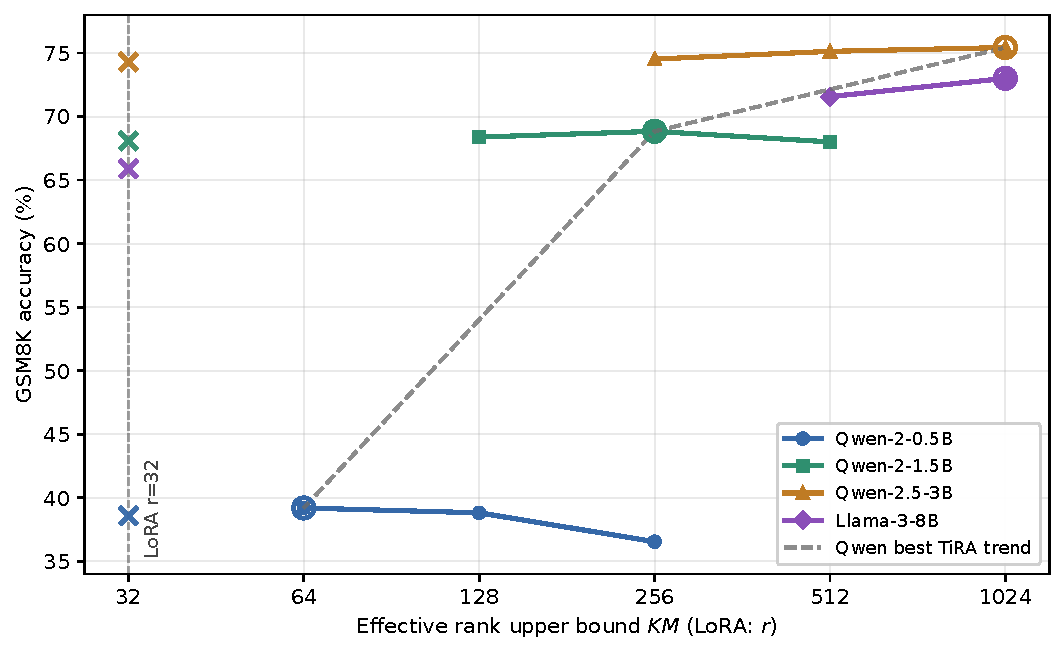
\includegraphics[width=0.88\linewidth]{figures/tira_ablation_m_trend.pdf}
    \caption{GSM8K accuracy of different models under LoRA and TiRA with different tiling granularities when $K=32$ is fixed. The horizontal axis denotes the effective rank upper bound. LoRA ($r=32$) is marked with a cross at 32 on the horizontal axis. Hollow circles mark the best TiRA configuration for each model, and the gray dashed line connects the best TiRA points of the Qwen series to highlight the rightward shift of the optimal tiling granularity as model scale increases.}
    \label{fig:ablation_m_trend}
\end{figure}

\paragraph{The optimal tiling granularity shifts rightward with model scale.}
Under the fixed budget $K=32$, the optimal $M$ shifts to larger values as model scale increases, and the ratio between the optimal equivalent rank and the hidden dimension also rises. The optimal $M$ values for Qwen-2-0.5B, Qwen-2-1.5B, and Qwen-2.5-3B are 2, 8, and 32, respectively, corresponding to total rank upper bounds $KM$ of 64, 256, and 1024. Compared with their hidden dimensions (896, 1536, and 2048), the ratio of the optimal equivalent rank to the hidden dimension increases from $7.1\%$ to $16.7\%$ and $50.0\%$. Figure~\ref{fig:ablation_m_trend} further shows that smaller models exhibit performance degradation at larger $M$, whereas larger models achieve their best results in higher effective-rank regions. Since this experiment fixes $K=32$ and TiRA requires $K\geq M$ with $K$ an integer multiple of $M$, the maximum tiling granularity considered here is $M=32$. The best result for Llama-3-8B appears at this search boundary, suggesting that larger $M$ is beneficial within the current experimental range, although further gains from larger $M$ under a higher $K$ budget cannot be ruled out. This trend indicates that larger models are more likely to support and benefit from higher-rank adaptation.

\paragraph{TiRA's structural advantage increases with model scale.}
Across the three Qwen models, the best TiRA configuration consistently outperforms the LoRA baseline, and the gain increases with model scale: Qwen-2-0.5B, Qwen-2-1.5B, and Qwen-2.5-3B improve by $0.61$, $0.76$, and $1.14$ percentage points, respectively. After adding Llama-3-8B, the improvement of the best TiRA configuration over LoRA ($r=32$) expands to $7.12$ percentage points. As shown in Fig.~\ref{fig:best_gain_scale}, the best TiRA gain generally increases with the hidden dimension. Notably, as the model scale grows, the fraction of trainable parameters decreases from $2.33\%$ to $0.70\%$, yet the relative gain of TiRA over LoRA still becomes larger. This suggests that TiRA's advantage mainly comes from structural high-rank expansion rather than from an increased parameter budget.

\begin{figure}[H]
    \centering
    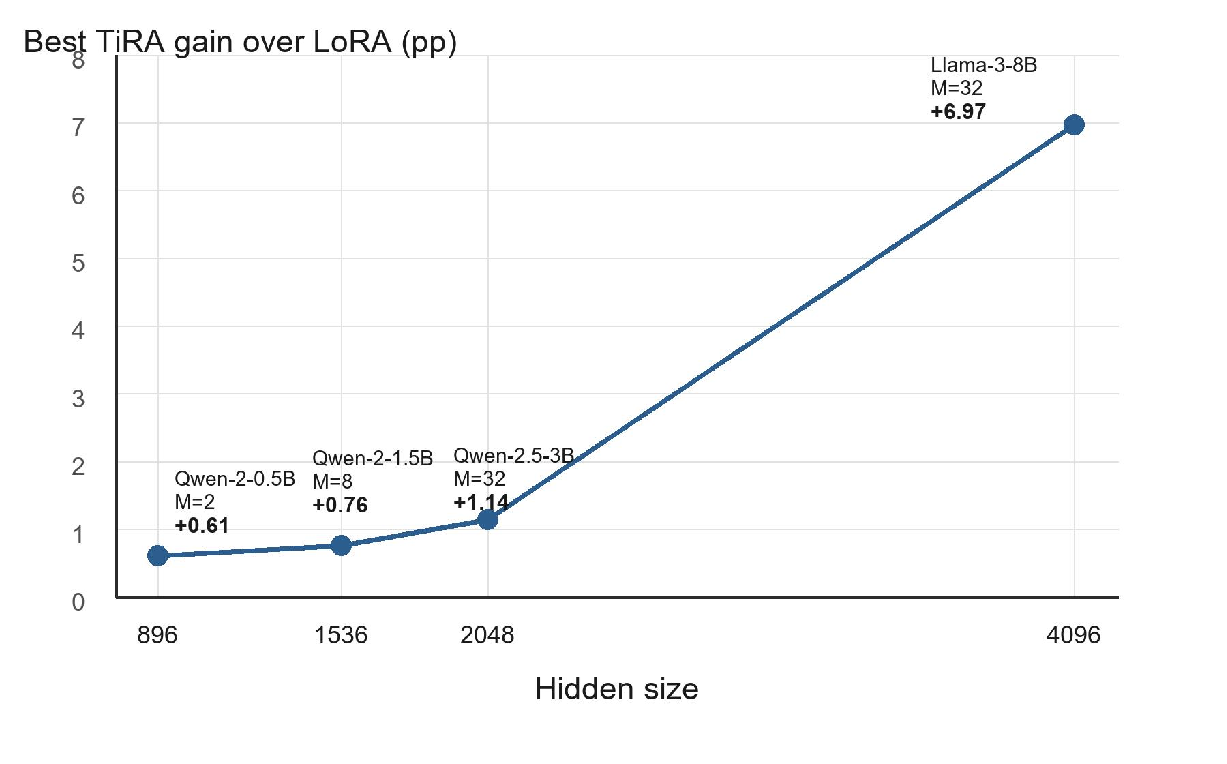
\includegraphics[width=0.82\linewidth]{figures/tira_best_gain_vs_scale.pdf}
    \caption{Accuracy gain of the best TiRA configuration over LoRA ($r=32$) across different model scales. The horizontal axis denotes the hidden dimension, and the vertical axis denotes the GSM8K accuracy difference between the best TiRA configuration and LoRA. The label beside each point gives the best tiling granularity $M$ within the current search range.}
    \label{fig:best_gain_scale}
\end{figure}

\paragraph{Excessive tiling granularity can lead to rank overload.}
TiRA's high-rank advantage does not monotonically improve as the grouping or tiling granularity $M$ increases; it is constrained by the base model's ability to support and coordinate the introduced perturbation directions. For Qwen-2-0.5B, accuracy already decreases when $M$ increases from 2 to 4, and further drops to $36.54\%$ at $M=8$, below the LoRA baseline of $38.59\%$. Qwen-2-1.5B also degrades at $M=16$, below its best configuration at $M=8$. This indicates that when the perturbation degrees of freedom introduced by TiRA exceed what the model can effectively coordinate, additional high-rank components do not necessarily improve adaptation and may instead degrade performance. We refer to this phenomenon as the rank-overload effect.

Larger models typically have higher hidden dimensions, stronger parameter redundancy, and richer representation spaces. Task-relevant features are more likely to be distributed across relatively separated subspaces, allowing multiple rank-1 components to act on different low-dimensional directions and be combined by optimization into a globally coherent high-rank perturbation. In contrast, smaller models have more limited representation spaces and adjustable degrees of freedom. When $M$ is too large, too many perturbation components may compete for the same or nearby feature channels, causing conflicts between gradient directions and stronger optimization coupling, which can offset the potential benefit of the higher-dimensional update space.

These observations reveal a coupling between tiling granularity and model scale. As model scale increases, representational redundancy and the number of perturbation directions that can be coordinated also increase, strengthening the model's ability to support high-rank adaptation. Therefore, whether high-rank updates are effective depends not only on whether the task requires a higher adaptation rank, but also on whether the base model can absorb such high-rank perturbations. The degradation on smaller models should not be simply attributed to failure of the TiRA structure. A more plausible interpretation is that $M$ simultaneously controls the degrees of freedom of high-rank perturbations and the difficulty of component coordination, and models of different scales differ in their ability to support these degrees of freedom. Thus, the optimal $M$ for TiRA should be matched to model scale and to the base model's ability to support high-rank perturbations. Larger models are more likely to benefit from larger $M$, whereas smaller models may enter the rank-overload regime once they exceed their support threshold, causing accuracy to decrease or even fall below the LoRA baseline.

\section{Conclusion}

This paper presents TiRA, a tiled high-rank parameter-efficient adaptation method for large language models. Under the same trainable-parameter scale as LoRA, TiRA uses structured tiling and shifted block-diagonal construction to expand the effective rank of weight updates from $r$ to $r^2$, thereby improving adaptation to complex reasoning and generation tasks. TiRA also preserves LoRA's mergeability and zero additional inference overhead. Extensive experiments show that, under matched parameter budgets, TiRA outperforms representative PEFT methods on commonsense reasoning, open-domain dialogue generation, and mathematical reasoning. Future work will further explore TiRA across more model scales, task types, and practical application scenarios, and will study more general matching principles among tiling granularity, model scale, and task complexity.

\begin{thebibliography}{99}

\bibitem{hu2022lora}
E. J. Hu, Y. Shen, P. Wallis, Z. Allen-Zhu, Y. Li, S. Wang, L. Wang, and W. Chen, ``LoRA: Low-rank adaptation of large language models,'' in \emph{Proc. Int. Conf. Learn. Represent. (ICLR)}, 2022.

\bibitem{wei2022cot}
J. Wei, X. Wang, D. Schuurmans, M. Bosma, B. Ichter, F. Xia, E. Chi, Q. Le, and D. Zhou, ``Chain-of-thought prompting elicits reasoning in large language models,'' in \emph{Adv. Neural Inf. Process. Syst.}, vol. 35, 2022, pp. 24824--24837.

\bibitem{kojima2022zero}
T. Kojima, S. S. Gu, M. Reid, Y. Matsuo, and Y. Iwasawa, ``Large language models are zero-shot reasoners,'' in \emph{Adv. Neural Inf. Process. Syst.}, vol. 35, 2022, pp. 22199--22213.

\bibitem{cobbe2021gsm8k}
K. Cobbe, V. Kosaraju, M. Bavarian, M. Chen, H. Jun, L. Kaiser, M. Plappert, J. Tworek, J. Hilton, R. Nakano, C. Hesse, and J. Schulman, ``Training verifiers to solve math word problems,'' \emph{arXiv preprint arXiv:2110.14168}, 2021.

\bibitem{liu2024dora}
S.-Y. Liu, C.-Y. Wang, H. Yin, P. Molchanov, Y.-C. F. Wang, K.-T. Cheng, and M.-H. Chen, ``DoRA: Weight-decomposed low-rank adaptation,'' in \emph{Proc. Int. Conf. Mach. Learn. (ICML)}, 2024.

\bibitem{jiang2024mora}
T. Jiang, S. Huang, S. Luo, Z. Zhang, H. Huang, F. Wei, W. Deng, F. Sun, Q. Zhang, D. Wang, and F. Zhuang, ``MoRA: High-rank updating for parameter-efficient fine-tuning,'' \emph{arXiv preprint arXiv:2405.12130}, 2024.

\bibitem{huang2025hira}
Q. Huang, T. Ko, Z. Zhuang, Y. Liu, Y. Wang, M. Hasegawa-Johnson, S. Watanabe, and Z. D. Chen, ``HiRA: Parameter-efficient Hadamard high-rank adaptation for large language models,'' in \emph{Proc. Int. Conf. Learn. Represent. (ICLR)}, 2025.

\bibitem{li2021prefix}
X. L. Li and P. Liang, ``Prefix-tuning: Optimizing continuous prompts for generation,'' in \emph{Proc. Joint Conf. ACL-IJCNLP}, 2021, pp. 4582--4597.

\bibitem{lester2021power}
B. Lester, R. Al-Rfou, and N. Constant, ``The power of scale for parameter-efficient prompt tuning,'' in \emph{Proc. Conf. Empir. Methods Nat. Lang. Process. (EMNLP)}, 2021, pp. 3045--3059.

\bibitem{xiao2022ptuning}
L. Xiao, K. Ji, and Y. Fu, ``P-tuning v2: Prompt tuning can be comparable to fine-tuning universally across scales,'' \emph{arXiv preprint arXiv:2110.07602}, 2022.

\bibitem{vaswani2017attention}
A. Vaswani, N. Shazeer, N. Parmar, J. Uszkoreit, L. Jones, A. N. Gomez, L. Kaiser, and I. Polosukhin, ``Attention is all you need,'' in \emph{Adv. Neural Inf. Process. Syst.}, vol. 30, 2017.

\bibitem{he2015rectifier}
K. He, X. Zhang, S. Ren, and J. Sun, ``Delving deep into rectifiers: Surpassing human-level performance on ImageNet classification,'' in \emph{Proc. IEEE Int. Conf. Comput. Vis. (ICCV)}, 2015, pp. 1026--1034.

\bibitem{hu2023llmadapters}
Z. Hu, L. Wang, Y. Lan, W. Xu, E.-P. Lim, L. Bing, X. Xu, S. Poria, and R. K.-W. Lee, ``LLM-Adapters: An adapter family for parameter-efficient fine-tuning of large language models,'' in \emph{Proc. Conf. Empir. Methods Nat. Lang. Process. (EMNLP)}, 2023, pp. 5254--5276.

\bibitem{bisk2019boolq}
Y. Bisk, C. Zelle, K. Lee, C. Chang, M. W. Chang, and K. Toutanova, ``BoolQ: Exploring the surprising difficulty of natural yes/no questions,'' in \emph{Proc. Conf. North Amer. Chapter Assoc. Comput. Linguistics: Human Lang. Technol. (NAACL-HLT)}, 2019, pp. 2924--2936.

\bibitem{bisk2020piqa}
Y. Bisk, R. Zellers, J. Gao, Y. Choi, \emph{et al.}, ``PIQA: Reasoning about physical commonsense in natural language,'' in \emph{Proc. AAAI Conf. Artif. Intell.}, vol. 34, no. 05, 2020, pp. 7432--7439.

\bibitem{sap2019socialiqa}
M. Sap, H. Rashkin, D. Chen, R. Le Bras, and Y. Choi, ``Social IQa: Commonsense reasoning about social interactions,'' in \emph{Proc. Conf. Empir. Methods Nat. Lang. Process. and Int. Joint Conf. Nat. Lang. Process. (EMNLP-IJCNLP)}, 2019, pp. 4463--4473.

\bibitem{zellers2019hellaswag}
R. Zellers, A. Holtzman, Y. Bisk, A. Farhadi, and Y. Choi, ``HellaSwag: Can a machine really finish your sentence?'' in \emph{Proc. Annu. Meeting Assoc. Comput. Linguistics (ACL)}, 2019, pp. 4791--4800.

\bibitem{sakaguchi2021winogrande}
K. Sakaguchi, R. L. Bras, C. Bhagavatula, and Y. Choi, ``WinoGrande: An adversarial Winograd schema challenge at scale,'' \emph{Commun. ACM}, vol. 64, no. 9, pp. 99--106, 2021.

\bibitem{clark2018arc}
P. Clark, I. Cowhey, O. Etzioni, T. Khot, A. Sabharwal, C. Schoenick, and O. Tafjord, ``Think you have solved question answering? Try ARC, the AI2 reasoning challenge,'' \emph{arXiv preprint arXiv:1803.05457}, 2018.

\bibitem{mihaylov2018openbookqa}
T. Mihaylov, P. Clark, T. Khot, and A. Sabharwal, ``Can a suit of armor conduct electricity? A new dataset for open book question answering,'' in \emph{Proc. Conf. Empir. Methods Nat. Lang. Process. (EMNLP)}, 2018, pp. 2381--2391.

\bibitem{dinan2019convai2}
E. Dinan, V. Logacheva, V. Malykh, A. H. Miller, K. Shuster, J. Urbanek, D. Kiela, A. Szlam, I. Serban, R. Lowe, S. Prabhumoye, A. W. Black, A. Rudnicky, J. Williams, J. Pineau, M. Burtsev, and J. Weston, ``The second conversational intelligence challenge (ConvAI2),'' in \emph{The NeurIPS'18 Competition: From Machine Learning to Intelligent Conversations}. Cham, Switzerland: Springer, 2019, pp. 187--208.

\bibitem{yu2024metamath}
L. Yu, W. Jiang, H. Shi, J. Yu, Z. Liu, Y. Zhang, J. T. Kwok, Z. Li, A. Weller, and W. Liu, ``MetaMath: Bootstrap your own mathematical questions for large language models,'' in \emph{Proc. Int. Conf. Learn. Represent. (ICLR)}, 2024.

\bibitem{papineni2002bleu}
K. Papineni, S. Roukos, T. Ward, and W.-J. Zhu, ``BLEU: A method for automatic evaluation of machine translation,'' in \emph{Proc. Annu. Meeting Assoc. Comput. Linguistics (ACL)}, 2002, pp. 311--318.

\bibitem{banerjee2005meteor}
S. Banerjee and A. Lavie, ``METEOR: An automatic metric for MT evaluation with improved correlation with human judgments,'' in \emph{Proc. ACL Workshop Intrinsic Extrinsic Eval. Measures Mach. Transl. Summarization}, 2005, pp. 65--72.

\bibitem{lin2004rouge}
C.-Y. Lin, ``ROUGE: A package for automatic evaluation of summaries,'' in \emph{Text Summarization Branches Out}, 2004, pp. 74--81.

\bibitem{zhang2019bertscore}
T. Zhang, V. Kishore, F. Wu, K. Q. Weinberger, and Y. Artzi, ``BERTScore: Evaluating text generation with BERT,'' \emph{arXiv preprint arXiv:1904.09675}, 2019.

\bibitem{touvron2023llama2}
H. Touvron, L. Martin, K. Stone, P. Albert, A. Almahairi, Y. Babaei, N. Bashlykov, S. Batra, P. Bhargava, S. Bhosale, \emph{et al.}, ``Llama 2: Open foundation and fine-tuned chat models,'' \emph{arXiv preprint arXiv:2307.09288}, 2023.

\bibitem{grattafiori2024llama3}
A. Grattafiori, A. Dubey, A. Jauhri, A. Pandey, A. Kadian, A. Al-Dahle, A. Letman, A. Mathur, A. Schelten, A. Vaughan, \emph{et al.}, ``The Llama 3 herd of models,'' \emph{arXiv preprint arXiv:2407.21783}, 2024.

\bibitem{yang2024qwen2}
A. Yang, B. Yang, B. Hui, B. Zheng, B. Yu, C. Zhou, C. Li, C. Li, D. Liu, F. Huang, \emph{et al.}, ``Qwen2 technical report,'' \emph{arXiv preprint arXiv:2407.10671}, 2024.

\bibitem{yang2024qwen25}
A. Yang, B. Yang, B. Zhang, B. Hui, B. Zheng, B. Yu, C. Li, D. Liu, F. Huang, H. Wei, \emph{et al.}, ``Qwen2.5 technical report,'' \emph{arXiv preprint arXiv:2412.15115}, 2024.

\end{thebibliography}

\appendix

\section{TiRA Construction Examples}

\subsection{\texorpdfstring{Block Construction with $K=M=3$}{Block Construction with K=M=3}}
\label{app:k3m3}

For $K=M=3$, the three adapter groups occupy three distinct cyclic-shift diagonals. Their sparse weight-update matrices can be written as
\begin{equation}
\Delta W_0=
\begin{bmatrix}
C_{0,0} & 0 & 0\\
0 & C_{0,1} & 0\\
0 & 0 & C_{0,2}
\end{bmatrix},\quad
\Delta W_1=
\begin{bmatrix}
0 & C_{1,0} & 0\\
0 & 0 & C_{1,1}\\
C_{1,2} & 0 & 0
\end{bmatrix},\quad
\Delta W_2=
\begin{bmatrix}
0 & 0 & C_{2,0}\\
C_{2,1} & 0 & 0\\
0 & C_{2,2} & 0
\end{bmatrix}.
\end{equation}
Here, $C_{k,m}\in\R^{(d_{\mathrm{out}}/M)\times(d_{\mathrm{in}}/M)}$ is the $m$-th rank-1 outer-product sub-block of the $k$-th adapter group along its cyclic-shift diagonal. The three groups complement each other along shifted block diagonals, and their sum creates nonzero sub-blocks at all $3\times3$ block positions:
\begin{equation}
\DeltaW=
\begin{bmatrix}
C_{0,0} & C_{1,0} & C_{2,0}\\
C_{2,1} & C_{0,1} & C_{1,1}\\
C_{1,2} & C_{2,2} & C_{0,2}
\end{bmatrix}.
\end{equation}

\subsection{Example of Multi-Sparse LoRA Expert Adaptation}
\label{app:sparse_expert}

For $d_{\mathrm{in}}=9$, $d_{\mathrm{out}}=9$, and $r=3$, the sparse weight-update matrices of LoRA expert adaptation can be written as follows.

The first group is the unshifted group, corresponding to $k=0$:
\[
\resizebox{\linewidth}{!}{$\displaystyle
\mathbf{B}_0 \mathbf{A}_0^\top =
\begin{bmatrix}
a_1 & 0 & 0 \\ 0 & a_2 & 0 \\ 0 & 0 & a_3 \\
b_1 & 0 & 0 \\ 0 & b_2 & 0 \\ 0 & 0 & b_3 \\
c_1 & 0 & 0 \\ 0 & c_2 & 0 \\ 0 & 0 & c_3
\end{bmatrix}
\begin{bmatrix}
m_1 & 0 & 0 & n_1 & 0 & 0 & o_1 & 0 & 0 \\
0 & m_2 & 0 & 0 & n_2 & 0 & 0 & o_2 & 0 \\
0 & 0 & m_3 & 0 & 0 & n_3 & 0 & 0 & o_3
\end{bmatrix}
=
\begin{bmatrix}
a_1 m_1 & 0 & 0 & a_1 n_1 & 0 & 0 & a_1 o_1 & 0 & 0 \\
0 & a_2 m_2 & 0 & 0 & a_2 n_2 & 0 & 0 & a_2 o_2 & 0 \\
0 & 0 & a_3 m_3 & 0 & 0 & a_3 n_3 & 0 & 0 & a_3 o_3 \\
b_1 m_1 & 0 & 0 & b_1 n_1 & 0 & 0 & b_1 o_1 & 0 & 0 \\
0 & b_2 m_2 & 0 & 0 & b_2 n_2 & 0 & 0 & b_2 o_2 & 0 \\
0 & 0 & b_3 m_3 & 0 & 0 & b_3 n_3 & 0 & 0 & b_3 o_3 \\
c_1 m_1 & 0 & 0 & c_1 n_1 & 0 & 0 & c_1 o_1 & 0 & 0 \\
0 & c_2 m_2 & 0 & 0 & c_2 n_2 & 0 & 0 & c_2 o_2 & 0 \\
0 & 0 & c_3 m_3 & 0 & 0 & c_3 n_3 & 0 & 0 & c_3 o_3
\end{bmatrix}
$}
\]

The second group applies a cyclic column shift by 1, corresponding to $k=1$:
\[
\resizebox{\linewidth}{!}{$\displaystyle
\mathbf{B}_1 \mathbf{A}_1^\top =
\begin{bmatrix}
e_1 & 0 & 0 \\ 0 & e_2 & 0 \\ 0 & 0 & e_3 \\
f_1 & 0 & 0 \\ 0 & f_2 & 0 \\ 0 & 0 & f_3 \\
g_1 & 0 & 0 \\ 0 & g_2 & 0 \\ 0 & 0 & g_3
\end{bmatrix}
\begin{bmatrix}
0 & q_2 & 0 & 0 & r_2 & 0 & 0 & s_2 & 0 \\
0 & 0 & q_3 & 0 & 0 & r_3 & 0 & 0 & s_3 \\
q_1 & 0 & 0 & r_1 & 0 & 0 & s_1 & 0 & 0
\end{bmatrix}
=
\begin{bmatrix}
0 & e_1 q_2 & 0 & 0 & e_1 r_2 & 0 & 0 & e_1 s_2 & 0 \\
0 & 0 & e_2 q_3 & 0 & 0 & e_2 r_3 & 0 & 0 & e_2 s_3 \\
e_3 q_1 & 0 & 0 & e_3 r_1 & 0 & 0 & e_3 s_1 & 0 & 0 \\
0 & f_1 q_2 & 0 & 0 & f_1 r_2 & 0 & 0 & f_1 s_2 & 0 \\
0 & 0 & f_2 q_3 & 0 & 0 & f_2 r_3 & 0 & 0 & f_2 s_3 \\
f_3 q_1 & 0 & 0 & f_3 r_1 & 0 & 0 & f_3 s_1 & 0 & 0 \\
0 & g_1 q_2 & 0 & 0 & g_1 r_2 & 0 & 0 & g_1 s_2 & 0 \\
0 & 0 & g_2 q_3 & 0 & 0 & g_2 r_3 & 0 & 0 & g_2 s_3 \\
g_3 q_1 & 0 & 0 & g_3 r_1 & 0 & 0 & g_3 s_1 & 0 & 0
\end{bmatrix}
$}
\]

The third group applies a cyclic column shift by 2, corresponding to $k=2$:
\[
\resizebox{\linewidth}{!}{$\displaystyle
\mathbf{B}_2 \mathbf{A}_2^\top =
\begin{bmatrix}
i_1 & 0 & 0 \\ 0 & i_2 & 0 \\ 0 & 0 & i_3 \\
j_1 & 0 & 0 \\ 0 & j_2 & 0 \\ 0 & 0 & j_3 \\
k_1 & 0 & 0 \\ 0 & k_2 & 0 \\ 0 & 0 & k_3
\end{bmatrix}
\begin{bmatrix}
0 & 0 & u_3 & 0 & 0 & v_3 & 0 & 0 & w_3 \\
u_1 & 0 & 0 & v_1 & 0 & 0 & w_1 & 0 & 0 \\
0 & u_2 & 0 & 0 & v_2 & 0 & 0 & w_2 & 0
\end{bmatrix}
=
\begin{bmatrix}
0 & 0 & i_1 u_3 & 0 & 0 & i_1 v_3 & 0 & 0 & i_1 w_3 \\
i_2 u_1 & 0 & 0 & i_2 v_1 & 0 & 0 & i_2 w_1 & 0 & 0 \\
0 & i_3 u_2 & 0 & 0 & i_3 v_2 & 0 & 0 & i_3 w_2 & 0 \\
0 & 0 & j_1 u_3 & 0 & 0 & j_1 v_3 & 0 & 0 & j_1 w_3 \\
j_2 u_1 & 0 & 0 & j_2 v_1 & 0 & 0 & j_2 w_1 & 0 & 0 \\
0 & j_3 u_2 & 0 & 0 & j_3 v_2 & 0 & 0 & j_3 w_2 & 0 \\
0 & 0 & k_1 u_3 & 0 & 0 & k_1 v_3 & 0 & 0 & k_1 w_3 \\
k_2 u_1 & 0 & 0 & k_2 v_1 & 0 & 0 & k_2 w_1 & 0 & 0 \\
0 & k_3 u_2 & 0 & 0 & k_3 v_2 & 0 & 0 & k_3 w_2 & 0
\end{bmatrix}
$}
\]

Summing the three groups gives the complete weight-update matrix:
\[
\resizebox{\linewidth}{!}{$\displaystyle
\Delta W_{\text{expert}}
= \frac{\alpha}{K}\left(\mathbf{B}_0 \mathbf{A}_0^\top+\mathbf{B}_1 \mathbf{A}_1^\top+\mathbf{B}_2 \mathbf{A}_2^\top\right)
= \frac{\alpha}{K}
\begin{bmatrix}
a_1 m_1 & e_1 q_2 & i_1 u_3 & a_1 n_1 & e_1 r_2 & i_1 v_3 & a_1 o_1 & e_1 s_2 & i_1 w_3 \\
i_2 u_1 & a_2 m_2 & e_2 q_3 & i_2 v_1 & a_2 n_2 & e_2 r_3 & i_2 w_1 & a_2 o_2 & e_2 s_3 \\
e_3 q_1 & i_3 u_2 & a_3 m_3 & e_3 r_1 & i_3 v_2 & a_3 n_3 & e_3 s_1 & i_3 w_2 & a_3 o_3 \\
b_1 m_1 & f_1 q_2 & j_1 u_3 & b_1 n_1 & f_1 r_2 & j_1 v_3 & b_1 o_1 & f_1 s_2 & j_1 w_3 \\
j_2 u_1 & b_2 m_2 & f_2 q_3 & j_2 v_1 & b_2 n_2 & f_2 r_3 & j_2 w_1 & b_2 o_2 & f_2 s_3 \\
f_3 q_1 & j_3 u_2 & b_3 m_3 & f_3 r_1 & j_3 v_2 & b_3 n_3 & f_3 s_1 & j_3 w_2 & b_3 o_3 \\
c_1 m_1 & g_1 q_2 & k_1 u_3 & c_1 n_1 & g_1 r_2 & k_1 v_3 & c_1 o_1 & g_1 s_2 & k_1 w_3 \\
k_2 u_1 & c_2 m_2 & g_2 q_3 & k_2 v_1 & c_2 n_2 & g_2 r_3 & k_2 w_1 & c_2 o_2 & g_2 s_3 \\
g_3 q_1 & k_3 u_2 & c_3 m_3 & g_3 r_1 & k_3 v_2 & c_3 n_3 & g_3 s_1 & k_3 w_2 & c_3 o_3
\end{bmatrix}
$}
\]

\subsection{\texorpdfstring{Multi-Layer Accumulation with $M=3,K=6$}{Multi-Layer Accumulation with M=3,K=6}}
\label{app:m3k6}

For $M=3,K=6$ ($L=2$), the 0-th diagonal band is produced jointly by groups 0 and 3, the 1-st diagonal band by groups 1 and 4, and the 2-nd diagonal band by groups 2 and 5. Corresponding block positions on the same diagonal band are summed, giving the total weight-update matrix
\begin{equation}
\DeltaW=
\begin{bmatrix}
C_{0,0}+C_{3,0} & C_{1,0}+C_{4,0} & C_{2,0}+C_{5,0}\\
C_{2,1}+C_{5,1} & C_{0,1}+C_{3,1} & C_{1,1}+C_{4,1}\\
C_{1,2}+C_{4,2} & C_{2,2}+C_{5,2} & C_{0,2}+C_{3,2}
\end{bmatrix}.
\end{equation}
Each unit block is now formed by summing two independent rank-1 outer products, increasing the within-block rank upper bound from 1 to 2.

\section{Hyperparameter Settings}

\subsection{LoRA Hyperparameters}
\label{app:lora_hyperparams}

\begin{table}[H]
\centering
\caption{LoRA hyperparameters for validating the relationship between task complexity and rank demand.}
\begin{tabular}{ll}
\toprule
Hyperparameter & Value \\
\midrule
Base Model & Qwen-2-1.5B \\
Method & LoRA \\
Datasets & GSM8K-Easy, GSM8K-Challenge \\
LoRA Rank ($r$) & 8, 16, 32, 64, 128 \\
LoRA Alpha ($\alpha$) & 8, 16, 32, 64, 128 \\
LoRA Dropout & 0.05 \\
Learning Rate & $1\times10^{-4}$ \\
Epochs & 2 \\
Batch Size & 160 \\
Warmup & 100 steps \\
Weight Decay & 0 \\
Target Modules & q\_proj, k\_proj, v\_proj, up\_proj, down\_proj \\
Evaluation Steps & Every 2 steps \\
\bottomrule
\end{tabular}
\end{table}

\subsection{TiRA Hyperparameters}
\label{app:tira_hyperparams}

\begin{table}[H]
\centering
\caption{TiRA hyperparameters used in the main experiments.}
\begin{tabular}{ll}
\toprule
Hyperparameter & Value \\
\midrule
Optimizer & AdamW \\
Weight Decay & 0 \\
Warmup & 100 steps \\
Batch Size & 32 \\
Target Modules & q\_proj, k\_proj, v\_proj, up\_proj, down\_proj \\
Evaluation Steps & Every 80 steps \\
\midrule
Commonsense Base Models & Llama-2-7B, Llama-3-8B \\
Commonsense $K,M$ & 32, 32 \\
Commonsense Learning Rate & $2\times10^{-4}$ \\
Commonsense Epochs & 2 \\
\midrule
Dialogue Base Model & Llama-3-8B \\
Dialogue $K,M$ & 32, 32 \\
Dialogue Learning Rate & $2\times10^{-5}$ \\
Dialogue Epochs & 1 \\
\midrule
Math Base Model & Llama-3-8B \\
Math $K,M$ & 32, 16/32 \\
Math Learning Rate & $4\times10^{-5}$ \\
Math Epochs & 2 \\
\bottomrule
\end{tabular}
\end{table}

\subsection{Tiling-Granularity Analysis Hyperparameters}
\label{app:ablation_hyperparams}

\begin{table}[H]
\centering
\caption{Hyperparameters for analyzing the effect of tiling granularity $M$ on TiRA adaptation performance.}
\begin{tabular}{ll}
\toprule
Hyperparameter & Value \\
\midrule
Dataset & MetaMath \\
Epochs & 2 \\
Batch Size & 32 \\
Warmup & 100 steps \\
Weight Decay & 0 \\
Target Modules & q\_proj, k\_proj, v\_proj, up\_proj, down\_proj \\
Evaluation Steps & Every 100 steps \\
\midrule
LoRA Rank/Alpha & 32/32 \\
LoRA Dropout & 0 \\
\midrule
TiRA Qwen-2-0.5B & $K=32$, $M\in\{2,4,8\}$, Learning Rate $1\times10^{-4}$ \\
TiRA Qwen-2-1.5B & $K=32$, $M\in\{4,8,16\}$, Learning Rate $7\times10^{-5}$ \\
TiRA Qwen-2.5-3B & $K=32$, $M\in\{16,32\}$, Learning Rate $5\times10^{-5}$ \\
\bottomrule
\end{tabular}
\end{table}

\end{document}
